\documentclass{article}

% Packages
\usepackage{packages}
\usepackage{commands}
\usepackage{titlepage}


% Title page parameters
\setUDK{612.8:[004.93+515.1]}
\setToResearch
\setTitle{Анализ аффективных компонентов ЭЭГ при прослушивании музыки}
\setGroup{207}
\setStudentSgn{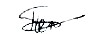
\includegraphics{my_sgn}}
\setStudent{А.С.Петелин}
\setStudentDate{18.05.2022}
\setAdvisor{Всеволод Леонидович Чернышев}
\setAdvisorTitle{доцент, к.ф.-м.н.}
\setAdvisorAffiliation{ФКН НИУ ВШЭ, Департамент больших данных и информационного поиска}
\setAdvisorDate{}
\setGrade{}
\setAdvisorSgn{}
\setYear{2022}


% Document Beginning
\begin{document}

\makeTitlePage

{
  \hypersetup{linkcolor=black}
  \tableofcontents
}

\hypersetup{linkcolor=black}

\section{Основные термины и определения}

% Возможно здесь необходимо будет привести ссылки на источники определений?

\textbf{Электроэнцефалограмма} (далее \textbf{ЭЭГ/EEG}) -- один из методов, позволяющих провести исследование головного мозга человека; в основе метода лежит регистрация электрических импульсов от мозга или каких-то его отдельных областей с помощью специального прибора.

\textbf{Центральная нервная система} (далее \textbf{ЦНС}) -- совокупность связанных между собой нейронов, у человека представлена головным и спинным мозгом.

\textbf{Отбор признаков / Feature Selection} (далее \textbf{FS}) -- это оценка значимости признаков модели с помощью алгоритмов машинного обучения с целью сокращения размерности исследуемого пространства.

\textbf{Метод главных компонент / Principle Component Analysis} (далее \textbf{PCA}) -- один из основных методов уменьшения размерности данных при минимизации потерь содержащейся в данных информации.

\textbf{Метод k-ближайших соседей / k-nearest neighbors} (далее \textbf{k-NN}) -- метрический алгоритм для автоматической классификации объектов или регрессии, основанный на оценивании сходства объектов.

\textbf{Метод опорных векторов / Support Vector Machine} (далее \textbf{SVM}) -- набор схожих алгоритмов обучения с учителем, использующихся для задач классификации и регрессионного анализа.

\textbf{Многослойный персептрон / Multilayered perceptron} (далее \textbf{MLP}) -- класс искусственных нейронных сетей, применимый в задачах классификации.

\textbf{Циркумплексная модель эмоций} -- предполагает, что эмоции распределяются в двумерном круговом пространстве, содержащем измерения возбуждения и привлекательности(валентности).

\textbf{Кросс-валидация} -- метод оценки аналитической модели и её поведения на независимых данных, основывающийся на разбиении данных на k частей.

\textbf{Датасет / Data Set} -- (размеченный) набор данных в табличном виде.

\textbf{DEAPdataset}~\cite{Koelstra},~\cite{DEAP} -- датасет для анализа эмоций с данными ЭЭГ, физиологических и видеосигналов.


\section{Введение}
Влияние музыки на слушателей отражено во многих источниках, как в художественных, так и в научных. Так, исследования показывают, что музыка помогает облегчить боль~\cite{Newbold}, влияет на координацию движений~\cite{Repp}~\cite{Aschersleben} и темпы дыхания~\cite{Siwiak}. Также одним из важнейших свойств музыки является её способность влиять на эмоциональное состояние человека~\cite{Koelsch}. Вопрос влияния на эмоциональное состояние человека является одним из ключевых при разработке систем взаимодействия человека и компьютера, более того, подбор подходящей музыки может улучшить состояние отдельного человека при использовании музыкального приложения~\cite{Leslie}. Примером компании, основавшей на этом позитивном изменении свою бизнес модель, является Endel~\cite{Endel}, разработавшая одноимённое приложение. Приложение предлагает персонализированные аудиотреки, которые ``помогут сосредоточиться, расслабиться и уснуть''.

Возрастающий интерес к музыкальной сфере как со стороны бизнеса, так и со стороны отдельных пользователей, позволяет говорить об актуальности изучения взаимодействия человека и музыки. Таким образом, можно поставить задачу распознавания влияния музыки на эмоциональное состояние человека. 

Для изучения влияния музыки прежде всего необходимо его измерить. В настоящий момент существует несколько технологий для фиксирования изменений эмоций, среди которых распознование эмоций по мимике (facial recognition), изучение переферийных физиологических сигналов, а также сигналов мозга. В данном иссследовании мы сосредоточимся на изучении данных о сигналах мозга, полученных с помощью ЭЭГ. Стоит отметить, что характеристики ЭЭГ содержат множество нелинейных зависимостей~\cite{Wang}, что позволяет в дальнейшем поставить вопрос об эффективности различных алгоритмов анализа данных. 

При переходе от этапа сбора данных к оцениванию, исследователи сталкиваются с рядом вопросов: как разбить данные? как сократить их размерность? каким образом классифицировать данные? Для решения этих проблем в машинном обучении существует множество подходов, одним из которых является PCA.

Метод PCA основан на поиске в исходном пространстве признаков гиперплоскости заданной размерности с последующим проектированием выборки на данную гиперплоскость. При этом выбирается та гиперплоскость, ошибка проектирования данных на которую является минимальной в смысле суммы квадратов отклонений. Метод позволяет не только сократить количество ключевых признаков, но и построить доступные проекции для оценки свойств данных.
При анализе данных ЭЭГ используется множество признаков, в связи с чем исследователи сталкиваются со значительным увеличением веса модели и времени её обучения, иногда сталкиваясь с проклятием размерности~\cite{Powell}. В таких условиях использование методов снижения размерности данных особенно важно. В данной работе будет рассмотрен алгоритм распознавания эмоций на основе датасета DEAP и продемонстрирована эффективность использования PCA при работе с большим количеством признаков. В соответствии с поставленной задачей можно выделить следующие цели исследования:
\begin{enumerate}
\item Подготовить данные на основе датасета DEAP;
\item Построить набор классификаторов для предсказывания эмоций в циркумплексной модели эмоций;
\item Использовать PCA как алгоритм FS для сокращения размерности пространства данных и выделения ключевых признаков будущей модели;
\item Сравнить эффективность использования классификаторов на исходной выборке и выборке, подвергнутой алгоритму PCA.
\end{enumerate}

Корректное использование метода PCA при анализе ЭЭГ позволит в дальнейшем получить преимущество как при иссследованиях, так и при разработке музыкальных сервисов.

\section{Обзор используемых источников}
Работа основана на исследовании открытого датасета DEAP, содержащего данные ЭЭГ и некоторые другие сведения, позволяющие изучать эмоции человека во время прослушивания музыки~\cite{Koelstra}. Сравнение некоторых алгоритмов отбора признаков, в том числе и PCA, для распознавания эмоций уже приведено в статье~\cite{Nawaz}, более того, авторы статей~\cite{Tandle}, \cite{Scherer} рассказывают ещё больше об исследовании данных ЭЭГ. Ряд авторов~\cite{Zhao}, ~\cite{Zheng} использует мультимодальные нейронные сети для достижения высокой точности предсказаний (state-of-art). Отдельные исследователи~\cite{Atkinson} применяют комбинацию качественного отбора признаков и необычного классификатора для повышения точности предсказаний на датасете DEAP. Представленные выше работы тесно связаны и находятся на переднем краю исследований в области анализа EEG данных, что предлагает серьёзную основу для данного исследования.

\section{Данные и методы}
\subsection{Модули Python}
Работа велась с использованием jyputer notebook~\cite{jyputer} (далее ноутбук), в который были загружены следующие библиотеки и модули:
\begin{enumerate}
\item Pandas -- для использования Dataframe, объекта для манипулирования индексированными массивами двумерных данных;
\item Seaborn и Matplotlib -- необходимые модули для визуализации данных, построения графиков;
\item Scipy -- импортируются функции для работы с данными ЭЭГ и математических преобразований, одна из ключевых функций -- signal.welch, позволяющая оценивать спектральную плотность сигнала с помощью метода Уэлча~\cite{Welch}.
\item Sklearn -- включает ключевые инструменты анализа данных, используемые в дальнейшем методы PCA, SVC, k-NN и MLP, а также метрики оценки качества обработки данных и построения классификаторов;
\item MNE -- используются модули для визуализации и кросс-валидации.
\end{enumerate}
Все используемые модули, включая стандартные, можно увидеть в секции 1.1. ноутбука.

\subsection{DEAP}
В проекте используются данные датасета DEAP, предназначенного для распознавания эмоций с использованием данных ЭЭГ, физиоологических и видеосигналов. С помощью специальных электродов, эти данные измерялись для 32 участников, каждый из которых посмотрел 40 одноминутных отрывков музыкальных клипов. Также частники оценивали каждый клип с точки зрения уровней возбуждения, валентности, доминирования и знакомства -- характеристик важных для распознавания эмоций, более подробно описанных в разделе Модель эмоций.

Стоит отметить, что данные датасета, используемые в проекте, уже прошли первичную обработку, в ходе которой были убраны артефакты и часть шумов. Чтобы получить доступ к данным, необходимо обратиться к авторам датасета на указанном выше сайте. В проект не включены данные датасета в соответствии с соглашением EULA, однако результаты работы можно воспроизвести, загрузив данные data\_preprocessed\_python.zip в папку project\_data.

Загрузка датасета происходит в секции 1.2. ноутбука. В данном проекте используются только данные с 32 датчиков ЭЭГ, а также шкалы Возбуждения(Arousal) и Валентности(Valence), выделение которых соответствует секциям 2.1. - 2.2. ноутбука.

\begin{figure}[h!]
\centering
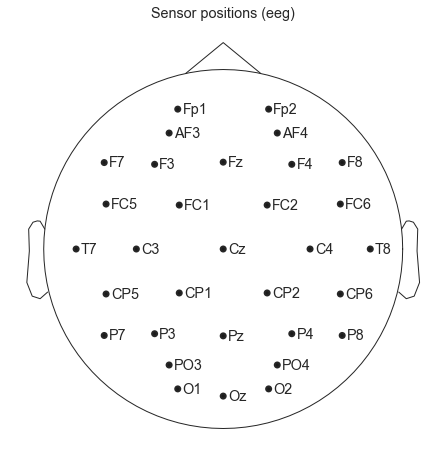
\includegraphics[scale=0.4]{channels.png}
\caption{Расположение датчиков на голове человека}
\end{figure}

\subsection{Модель эмоций}
Исследование опирается на использование циркумплексной модели эмоций, предложенной Джеймсом Расселом~\cite{Russell}. Модель основывается на распределении эмоций в двумерном круговом пространстве, содержащем измерения возбуждения и валентности. Возбуждение представляет собой вертикальную ось, а валентность представляет собой горизонтальную ось, а центр круга представляет нейтральную валентность и средний уровень возбуждения. Различные чёткие эмоции могут быть нанесены на циркумплекс в соответствии с их уровнями возбуждения и валентности.

\begin{figure}[h!]
\centering
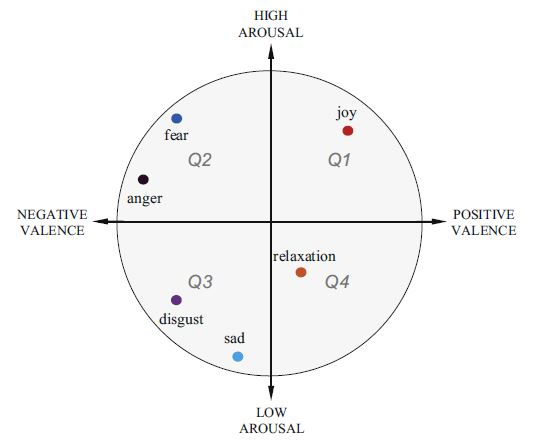
\includegraphics[scale=0.5]{emotions.JPG}
\caption{Четкие эмоции на циркумплексе Рассела~\cite{balanzo}}
\end{figure}

В исследовании показатели возбуждения и валентности кодируются бинарно относительно медианы измерений. Таким образом, каждый прослушанный клип имеет бинарный рейтинг по каждой шкале, что позволяет сформировать 4 категории эмоций, соответствующих четвертям циркумплекса:
\begin{enumerate}
    \item Высокое Возбуждение, Высокая Валентность / High Arousal High Valence (далее HAHV)
    \item Низкое Возбуждение, Высокая Валентность / Low Arousal High Valence (далее LAHV)
    \item Высокое Возбуждение, Низкая Валентность / High Arousal Low Valence (далее HALV)
    \item Низкое Возбуждение, Низкая Валентность / Low Arousal Low Valence (далее LALV)
\end{enumerate}
Эти категории также добавлены в датафрейм и закодированы в секции 2.1. ноутбука, распределение возбуждения и валентности в четвертях циркумплекса можно наблюдать на изображении ниже.

\begin{figure}[h]
\centering
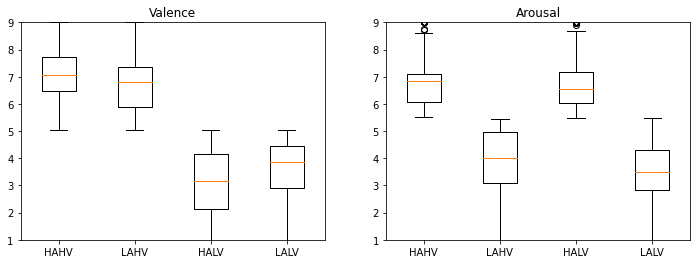
\includegraphics[scale=0.5]{valence_arousal.png}
\caption{Распределение Возбуждения(Arousal) и Валентности(Valence) относительно четвертей циркумплекса}
\end{figure}

\section{Работа с данными}
\subsection{Извлечение признаков}
Как уже было отмечено, в исследовании рассматриваются только данные 32 датчиков ЭЭГ для каждого клипа. В соответствии с этим, для каждого сигнала можно выделить следующие категории признаков:
\begin{enumerate}
    \item Мощности частотных диапазонов;
    \item Статистические характеристики;
    \item Параметры Хьорта~\cite{Hjorth};
    \item Фрактальная размерность.
\end{enumerate}
Опишем введённые параметры.
\subsubsection{Мощности частотных диапазонов}
Рассмотрим сырые данные из датасета.

\begin{figure}[h]
\centering
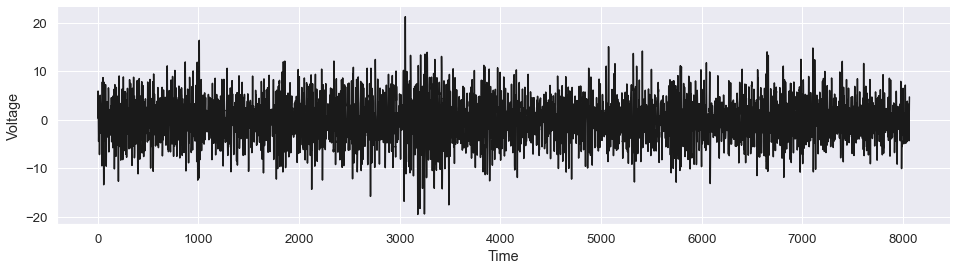
\includegraphics[scale=0.5]{signal.png}
\caption{Сигнал}
\end{figure}

Как можно понять по графику, на протяжении времени измеряется только напряжение. Однако напряжения недостаточно для характеристики мозговых волн, в связи с чем вводится дополнительная характеристика -- спектральная плотность мощности. СПМ -- функция, описывающая распределение мощности сигнала в зависимости от частоты. Её можно вычислить методом Уэлча\cite{Welch}.
Пример вычисления такой характеристики для отдельного сигнала можно увидеть на изображении ниже.

\begin{figure}[h]
\centering
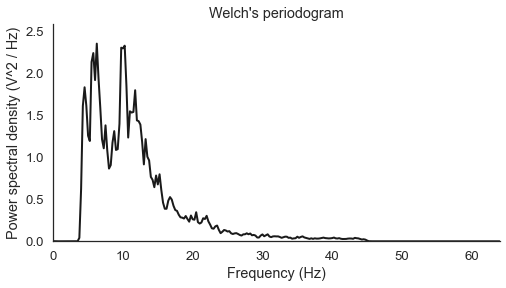
\includegraphics[scale=0.5]{welch.png}
\caption{Периодограмма Уэлча}
\end{figure}

Однако напрямую данная характеристика в исследовании не будет использоваться, но понадобится для вычисления средней мощности входного сигнала (bandpower), которую мы вычислим для каждого диапазона частот мозга.

При передаче электрических импульсов по нервным волокнам от нейрона к нейрону мозг человека генерирует волны, называемые мозговыми. Они принимают значения от 1 до 70 Гц и выше и подразделяются на следующие категории:

\setlength{\tabcolsep}{18pt}
\renewcommand{\arraystretch}{1.5}

\paragraph{}
\begin{tabular}{|m{5cm}|m{5cm}|}
    \hline
    \textbf{Название диапазона} & \textbf{Принимаемые значения}\\
    \hline
    Дельта-волны & 1 - 4 Гц\\
    \hline
    Тета-волны & 4 - 8 Гц\\
    \hline
    Альфа-волны & 8 - 12 Гц\\
    \hline
    Бета-волны & 12 - 30 Гц\\
    \hline
    Гамма-волны & 30 - 70 Гц\\
    \hline  
\end{tabular}
\paragraph{}

Стоит отметить, что датчики не замеряли дельта-волны, а гамма-волны были ограничены сверху в 64 Гц. После разбиения частот на диапазоны для каждого из 4 диапазонов(дельта, тета, альфа и гамма) необходимо вычислить соответствующую мощность сигнала. Вычисление реализовано на основе алгоритма, предложенного Raphael Vallat\cite{Vallat}.


\subsubsection{Статистические характеристики}
Изначально предполагалось использование 6 характеристик -- функций от массива значений напряжения конкретного электрода: медиана, среднее, максимальное и минимальное значение, стандартное отклонение и коэффициент эксцесса (Куртосис). Однако в ходе работы я ограничился тремя из них:
\begin{enumerate}
\item Среднее (арифметическое) -- мера центральной тенденции, равная сумме всех чисел множества, делённой на их количество:
$$\bar{x} = \frac{1}{n}\sum_{i=1}^n x_i  =  \frac{1}{n} (x_1+\cdots+x_n)$$
\item Стандартное отклонение -- мера величины вариации или дисперсии набора значений. Определяется как корень из дисперсии случайной величины:
$$\sigma = \sqrt{\mathrm{D}[X]}$$
\item Куртосис -- мера остроты пика распределения случайной величины~\cite{Kurtosis}. Определяется следующим образом для случайной величины $X$, такой что $\mathbb{E}|X|^4 < \infty$. Пусть $\mu_4$ обозначает четвёртый центральный момент $X$, а $\sigma$ - стандартное отклонение $X$, тогда куртосис вычисляется как $$\gamma_2 = \frac{\mu_4}{\sigma^4} - 3$$

\end{enumerate}
\subsubsection{Параметры Хьорта}
Данные параметры были предложены Бо Хьортом~\cite{Hjorth} для исследования данных ЭЭГ, на эти признаки опирались некоторые представленные в библиографии статьи.
\begin{enumerate}
\item Активность -- представляет мощность сигнала, дисперсию временной функции~\cite{Hjorth_defs}:
$$\text{Activity}  =  \text{var}(y(t))$$

\item Мобильность -- представляет собой среднюю частоту или долю стандартного отклонения спектра мощности и определяется как квадратный корень из дисперсии первой производной сигнала, деленной на дисперсию сигнала~\cite{Hjorth_defs}:
$$\text{Mobility} =\sqrt\frac{{\text{var}(\frac{dy(t)}{dt})}}{\text{var}(y(t))}$$

\item Сложность -- представляет изменение частоты~\cite{Hjorth_defs} и выражается следующим образом:
$$\text{Complexity} =\frac{{\text{Mobility}(\frac{dy(t)}{dt})}}{\text{Mobility}(y(t))}$$
\end{enumerate}
\subsubsection{Фрактальная размерность}
Используется параметр фрактальной размерности, предложенный А.Петросяном~\cite{Petrosian} и вычисляющийся как
$$P = \frac{\log_{10}(N)}{\log_{10}(N) +
\log_{10}(\frac{N}{N+0.4N_{\delta}})}$$
где $N$ -- длина сигнала, а $N_{\delta}$ является числом изменений знака в производной сигнала.

\paragraph{} Помимо введённых параметров, в исследованиях ЭЭГ также используются другие характеристики, такие как логарифмические мощности частотных диапазонов~\cite{Brunner} и Вейвлет-преобразование~\cite{Petrantonakis}.

Вычислив параметры в секции 3.1. ноутбука, был получен датафрейм, содержащий 11 характеристик каждого из 32 сигналов, всего 352 признака.

\begin{figure}[h]
\centering
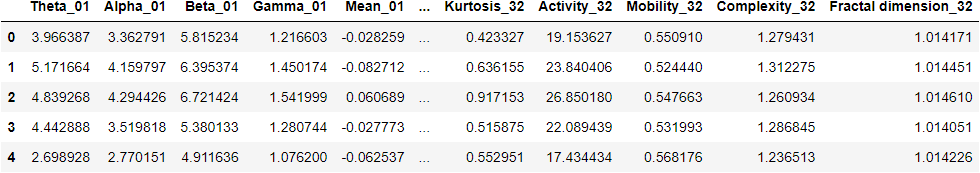
\includegraphics[scale=0.65]{df_x.png}
\caption{Фрагмент датафрейма}
\end{figure}

\subsection{Классификация}
Нас будет интересовать задача классификации клипов по типу вызываемых эмоций. В фокусе внимания находится предсказание возбуждения (высокого или низкого), валентности (высокой или низкой), а также четверти циркумплекса (HAHV, LAHV, HALV, LALV) в предложенной ранее модели эмоций.
Для обработки полученного набора признаков будем разбивать данные на тренировочную и тестовую выборки, а затем проводить Маштабирование признаков (Feature Scaling) как предложено в секции 5.1 ноутбука. Маштабирование признаков помогает нормализовать выборку, что существенно для работы некоторых классификаторов. Далее используем несколько классификаторов, применив подход кросс-валидации с 5-кратной проверкой (kFold=5). В проекте использованы классификаторы SVM, k-NN и MLP.

Будем отслеживать точность предсказаний для 3 признаков, упомянутых выше: Arousal(1, 0), Valence(1, 0) и State(HAHV, LAHV, HALV, LALV).
После описанной процедуры были получены следующие точности(секция 3.2 ноутбука):
\begin{itemize}
\item Точность для Arousal: 64.23;
\item Точность для Valence: 67.48;
\item Точность для State: 43.9.
\end{itemize}
Несмотря на точность, сопоставимую с результатами статьи~\cite{Atkinson}, с помощью применения PCA можно добиться улучшения точности.

\subsection{Применение PCA}
Как в предыдущем случае, сначала произведём маштабирование признаков (секция 4.1 ноутбука), так как оно существенно для корректной работы алгоритма PCA. Затем напишем функцию, которая будет использовать PCA с заданным числом компонент(секция 4.2 ноутбука).
Чтобы вычислить оптимальное число компонент, применим PCA для всех размеров компонент в диапазоне от 2 до 75 (до четверти от исходного количества признаков -- 352).
После каждого применения PCA применим функцию для измерения точности предсказания с предложенными классификаторами из пункта выше и построим график, сопоставляющий число компонент PCA с точностью предсказаний (секция 5.3 ноутбука).

\begin{figure*}[h!]
    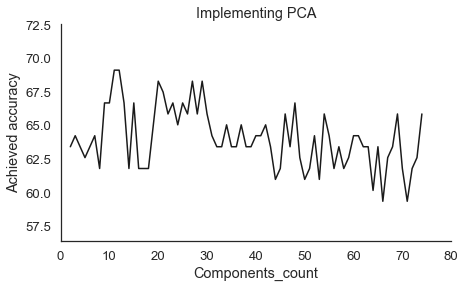
\includegraphics[width=.3\textwidth]{arousal_pca.png}\hfill
    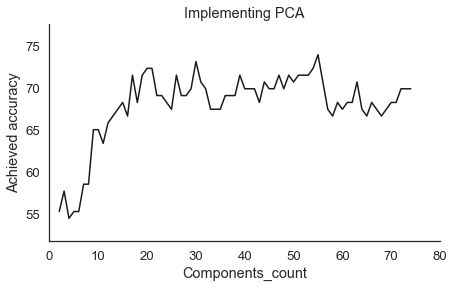
\includegraphics[width=.3\textwidth]{valence_pca.png}\hfill
    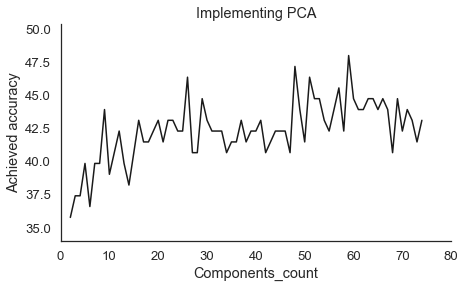
\includegraphics[width=.3\textwidth]{state_pca.png}
    \caption{Применение PCA для предсказания Arousal, Valence и State}
\end{figure*}
    
    
\paragraph{}
По графику видно, что даже при малом числе компонент можно добиться высокой точности модели.
В соответствии с графиком выберем небольшое, оптимальное число компонент и оценим точность предсказаний.
\begin{itemize}
\item Улучшение точности предсказания для Arousal после PCA: 64.23 -> 69.11 . Всего: + 4.88\%;
\item Улучшение точности предсказания для Valence после PCA: 67.48 -> 73.17 . Всего: + 5.69\%;
\item Улучшение точности предсказания для State после PCA: 43.9 -> 49.59 . Всего: + 5.69\%.
\end{itemize}

Также можно оценить снижение количества компонент

\begin{itemize}
\item Достигнутая точность для Arousal: 69.11 . Снижение числа компонент:  352  ->  12;
\item Достигнутая точность для  Valence: 73.17 . Снижение числа компонент:  352  ->  30;
\item Достигнутая точность для State: 49.59 . Снижение числа компонент:  352  ->  59.
\end{itemize}

\section{Полученные результаты}
\subsection{Сравнение результатов классификации с использованием PCA - секция 5.4}
Рассмотрев полученные результаты (секция 5.4 ноутбука), можно выявить преимущества использования PCA над выборкой перед классификацией. Прежде всего, это многократное сокращение количества признаков, необходимых для точной работы модели. Более того, в результате преобразований были получены такие признаки, что точность модели даже повысилась (в среднем, на 5 процентных пунктов). Это может свидетельствовать о применимости PCA в очистке шума и лишних признаков, которые могли ухудшать качество модели.
При исследованиях ЭЭГ как сокращение количества признаков модели, так и очистка шума являются важными задачами. Проведённое исследование демонстрирует эффективность PCA в решении этих задач и доказывает применимость PCA в повышении точности модели и сокращения её веса.

\subsection{Рассуждения}
Тем не менее, существуют другие способы отбора признаков, например, в уже упомянутой статье~\cite{Atkinson} используется алгоритм Максимальной релевантности -- минимальной избыточности / Maximum Relevance — Minimum Redundancy(MRMR) и достигаются аналогичные результаты. Некоторые исследователи используют Анализ независимых компонент / Independent component analysis (ICA) для отбора признаков модели. Более того, на передний план выходит необходимость выявления нелинейных зависимостей признаков~\cite{Wang}, для чего PCA неприменима, в связи с чем используются модели, основанные на глубоких нейронных сетях. Использование мультимодальных нейронных сетей было успешно в статьях~\cite{Zhao}, ~\cite{Zheng}, являющиеся state-of-the-art работами, основанными также на данных DEAP. Все указанные способы отбора признаков отличаются от рассмотреного в исследовании, что позволяет говорить о необходимости выявления наиболее оптимальных подходов в будущем.

% Bibliography
\bibliographystyle{unsrt}
\bibliography{bibl}

\section*{Приложение A. Цифровые материалы}
Ноутбук, а также .tex файлы для формирования документа и иллюстрации можно найти на

\url{https://github.com/chmousNedovolniy/ResearchProject}. 

\end{document}
